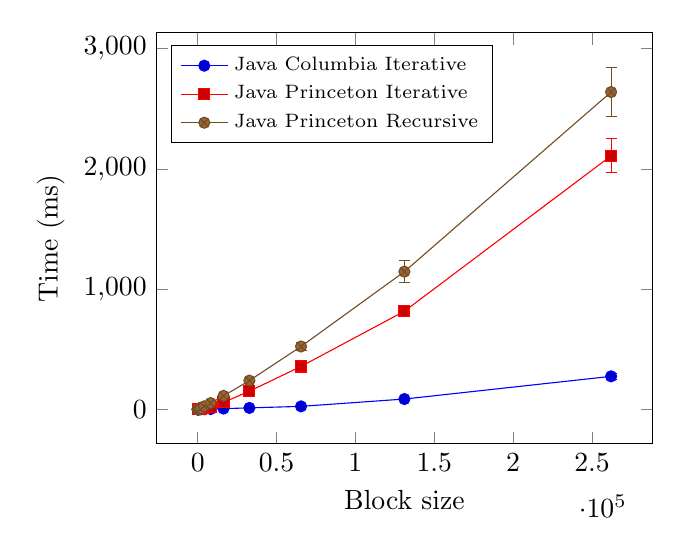
\begin{tikzpicture}
\begin{axis}[xlabel={Block size},ylabel={Time (ms)},width=0.65\linewidth,legend pos=north west,scaled y ticks = false,legend cell align=left,legend style={font=\scriptsize}]
\addplot+[error bars/.cd, y dir=both,y explicit] coordinates {
(16, 0.0370) +- (0.0055, 0.0055)
(32, 0.0899) +- (0.0169, 0.0169)
(64, 0.0244) +- (0.0637, 0.0637)
(128, 0.0134) +- (0.0005, 0.0005)
(256, 0.0293) +- (0.0042, 0.0042)
(512, 0.0615) +- (0.0047, 0.0047)
(1024, 0.1484) +- (0.0308, 0.0308)
(2048, 0.4338) +- (0.0806, 0.0806)
(4096, 1.2071) +- (0.1807, 0.1807)
(8192, 2.8726) +- (0.3247, 0.3247)
(16384, 6.3214) +- (1.0542, 1.0542)
(32768, 12.2634) +- (2.9076, 2.9076)
(65536, 24.9874) +- (4.6266, 4.6266)
(131072, 85.9483) +- (8.2128, 8.2128)
(262144, 274.5134) +- (26.0859, 26.0859)
};
\addplot+[error bars/.cd, y dir=both,y explicit] coordinates {
(16, 0.1227) +- (0.0268, 0.0268)
(32, 0.1392) +- (0.6110, 0.6110)
(64, 0.0905) +- (0.2393, 0.2393)
(128, 0.1431) +- (0.0097, 0.0097)
(256, 0.5698) +- (0.4834, 0.4834)
(512, 0.8758) +- (0.3145, 0.3145)
(1024, 1.7488) +- (0.3452, 0.3452)
(2048, 4.4055) +- (1.0527, 1.0527)
(4096, 9.6792) +- (2.3947, 2.3947)
(8192, 22.9609) +- (5.6248, 5.6248)
(16384, 58.3825) +- (9.9410, 9.9410)
(32768, 150.7299) +- (5.5432, 5.5432)
(65536, 356.9871) +- (8.0942, 8.0942)
(131072, 815.8607) +- (17.5017, 17.5017)
(262144, 2108.0771) +- (140.4932, 140.4932)
};
\addplot+[error bars/.cd, y dir=both,y explicit] coordinates {
(16, 0.1304) +- (0.0546, 0.0546)
(32, 0.0670) +- (0.0177, 0.0177)
(64, 0.1352) +- (0.0215, 0.0215)
(128, 0.4913) +- (0.2475, 0.2475)
(256, 0.6929) +- (0.1662, 0.1662)
(512, 1.7515) +- (0.6352, 0.6352)
(1024, 3.7688) +- (1.1879, 1.1879)
(2048, 8.6983) +- (2.3341, 2.3341)
(4096, 25.0276) +- (4.3322, 4.3322)
(8192, 52.0853) +- (7.1292, 7.1292)
(16384, 112.3024) +- (8.1890, 8.1890)
(32768, 239.0777) +- (12.8962, 12.8962)
(65536, 522.7409) +- (31.4586, 31.4586)
(131072, 1144.8802) +- (91.1919, 91.1919)
(262144, 2638.0547) +- (206.8494, 206.8494)
};
\legend{Java Columbia Iterative , Java Princeton Iterative , Java Princeton Recursive}
\end{axis}
\end{tikzpicture}
